\renewcommand*{\arraystretch}{1.1}

\label{sec:bi-read-15}
\noindent\begin{tabularx}{\queryCardWidth}{|>{\queryPropertyCell}c|X|}
	\hline
	query & BI / read / 15 \\ \hline
%
	title & Social normals \\ \hline
%
    pattern & \hfill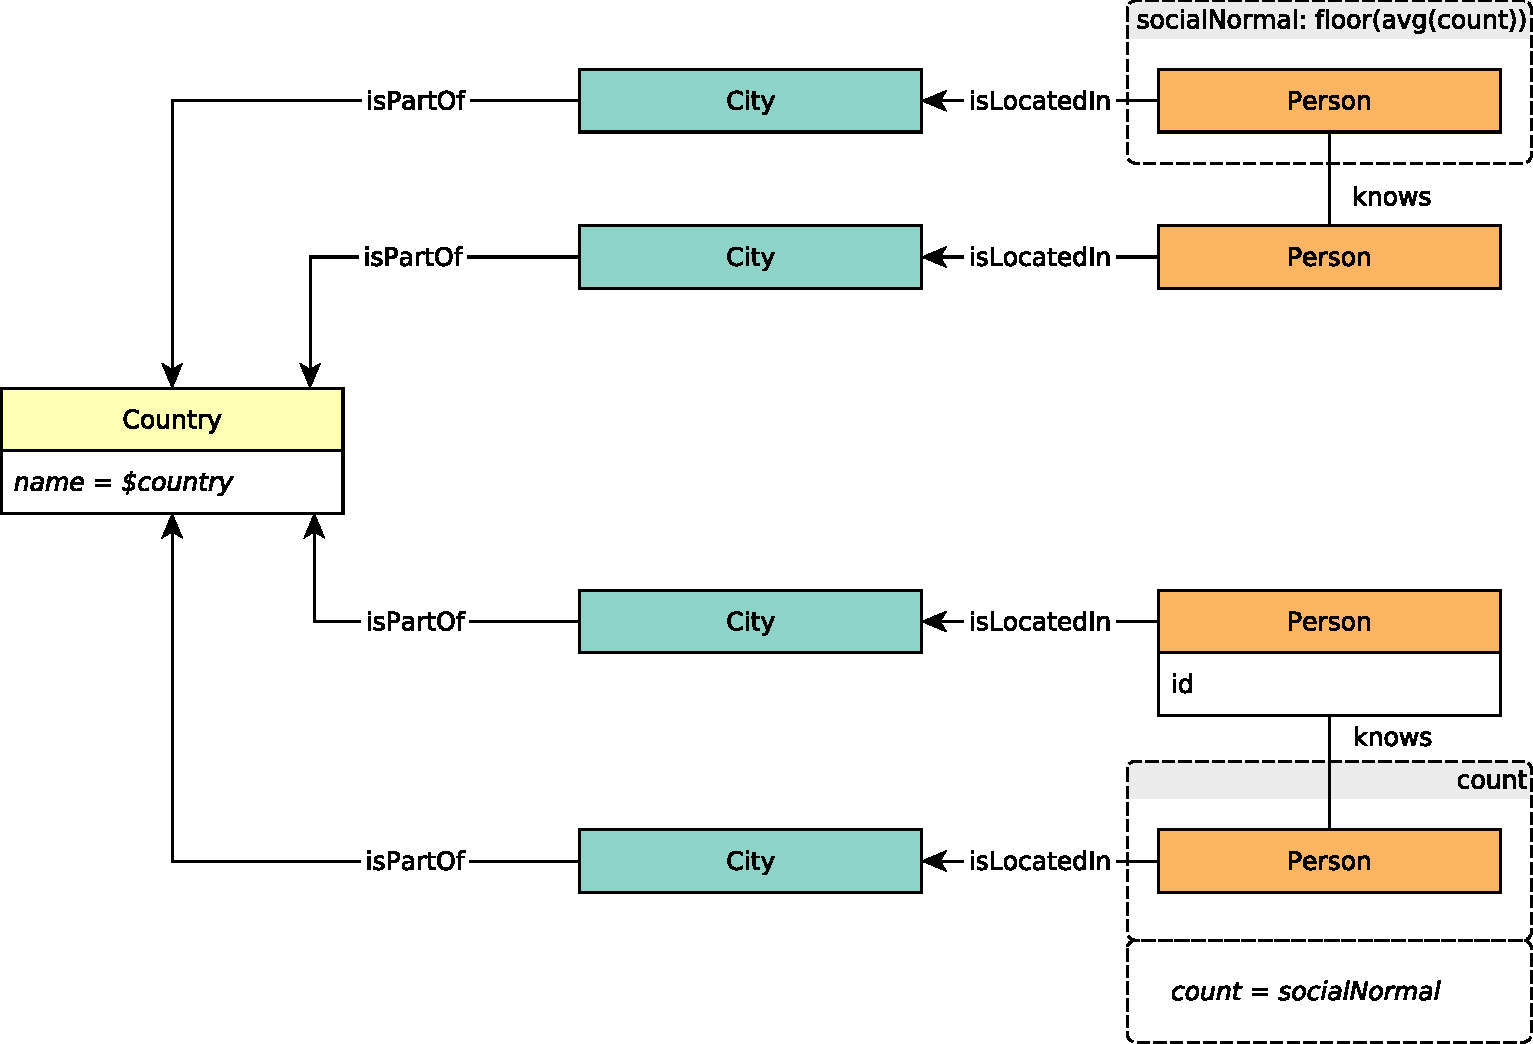
\includegraphics[scale=\patternscale,margin=0cm .2cm]{patterns/bi-read-15}\hfill\vadjust{} \\ \hline
%
	desc. & Given a country, find all Persons of the country whose number of friends
in the given country equals the (floor of) average number of friends
that Persons of the given country have in the given country.
 \\ \hline
%
	
%
    
        params &
        \innerCardVSpace{\begin{tabularx}{\attributeCardWidth}{|>{\paramNumberCell}c|>{\varNameCell}M|>{\typeCell}m{\typeWidth}|Y|} \hline
        \cellcolor{parameter} \color{white} \footnotesize $\mathsf{1}$ &country& 32-bit Integer &  \\ \hline
        \end{tabularx}}\innerCardVSpace \\ \hline
	
%
	
        result &
        \innerCardVSpace{\begin{tabularx}{\attributeCardWidth}{|>{\resultNumberCell}c|>{\varNameCell}M|>{\typeCell}m{\typeWidth}|>{\resultOriginCell}c|Y|} \hline
        $\mathsf{1}$ & person.id & 64-bit Integer &R&
                 \\ \hline
        $\mathsf{2}$ & count & 32-bit Integer &A&
                 \\ \hline
        \end{tabularx}}\innerCardVSpace \\ \hline
	
%
	sort        &
        \innerCardVSpace{\begin{tabular}{|>{\sortNumberCell}c|>{\varNameCell}l|>{\directionCell}c|} \hline
        $\mathsf{1}$ & person.id & $\asc$ \\ \hline
        \end{tabular}}\innerCardVSpace \\ \hline
	%
	limit & 100 \\ \hline
	%
	CPs &
	\multicolumn{1}{>{\raggedright}l|}{
	    \chokePoint{1.2}, 
	    \chokePoint{2.3}, 
	    \chokePoint{3.2}, 
	    \chokePoint{3.3}, 
	    \chokePoint{5.3}, 
	    \chokePoint{6.1}
	    } \\ \hline
	%
    %
\end{tabularx}
\queryCardVSpace